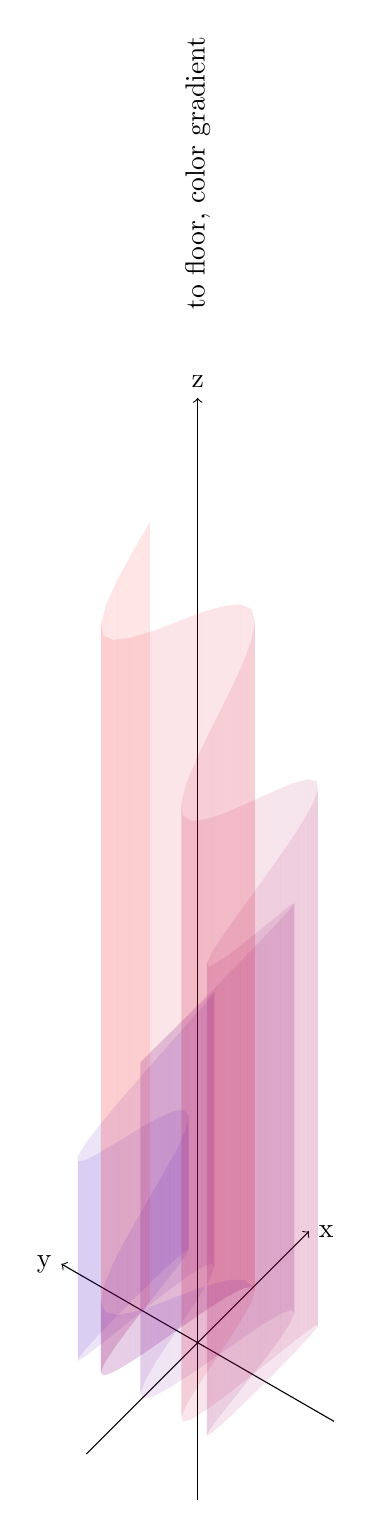
\begin{tikzpicture}[
  x={(0.707cm,0.707cm)},
  z={(0cm,1cm)},
  y={(-0.866cm,0.5cm)}]

  \draw[->] (-2,0,0) -- (2,0,0) node[right] {x};
  \draw[->] (0,-2,0) -- (0,2,0) node[left] {y};
  \draw[->] (0,0,-2) -- (0,0,12) node[above] {z};
  \foreach \z in {0,0.1,...,9.9}{
    \pgfmathtruncatemacro{\mycolorpercentage}{\z/0.099}
    \fill[red!\mycolorpercentage!blue,opacity=0.1]
      ({cos(\z*210)},{sin(\z*42)},0) --
      ({cos(\z*210)},{sin(\z*42)},{\z}) --
      ({cos((\z+0.1)*210)},{sin((\z+0.1)*42)},{\z+0.1}) --
      ({cos((\z+0.1)*210)},{sin((\z+0.1)*42)},0) -- cycle;
  }
  \node[rotate=90,right=1cm] at (0,0,12) {to floor, color gradient};
\end{tikzpicture}
